%Version 2.1 April 2023
% See section 11 of the User Manual for version history
%
%%%%%%%%%%%%%%%%%%%%%%%%%%%%%%%%%%%%%%%%%%%%%%%%%%%%%%%%%%%%%%%%%%%%%%
%%                                                                 %%
%% Please do not use \input{...} to include other tex files.       %%
%% Submit your LaTeX manuscript as one .tex document.              %%
%%                                                                 %%
%% All additional figures and files should be attached             %%
%% separately and not embedded in the \TeX\ document itself.       %%
%%                                                                 %%
%%%%%%%%%%%%%%%%%%%%%%%%%%%%%%%%%%%%%%%%%%%%%%%%%%%%%%%%%%%%%%%%%%%%%

%%\documentclass[referee,sn-basic]{sn-jnl}% referee option is meant for double line spacing

%%=======================================================%%
%% to print line numbers in the margin use lineno option %%
%%=======================================================%%

%%\documentclass[lineno,sn-basic]{sn-jnl}% Basic Springer Nature Reference Style/Chemistry Reference Style

%%======================================================%%
%% to compile with pdflatex/xelatex use pdflatex option %%
%%======================================================%%

%%\documentclass[pdflatex,sn-basic]{sn-jnl}% Basic Springer Nature Reference Style/Chemistry Reference Style


%%Note: the following reference styles support Namedate and Numbered referencing. By default the style follows the most common style. To switch between the options you can add or remove “Numbered” in the optional parenthesis. 
%%The option is available for: sn-basic.bst, sn-vancouver.bst, sn-chicago.bst, sn-mathphys.bst. %  


 
%%\documentclass[sn-nature]{sn-jnl}% Style for submissions to Nature Portfolio journals
%%\documentclass[sn-basic]{sn-jnl}% Basic Springer Nature Reference Style/Chemistry Reference Style
\documentclass[sn-mathphys,Numbered]{sn-jnl}% Math and Physical Sciences Reference Style
%%\documentclass[sn-aps]{sn-jnl}% American Physical Society (APS) Reference Style
%%\documentclass[sn-vancouver,Numbered]{sn-jnl}% Vancouver Reference Style
%%\documentclass[sn-apa]{sn-jnl}% APA Reference Style 
%%\documentclass[sn-chicago]{sn-jnl}% Chicago-based Humanities Reference Style
%%\documentclass[default]{sn-jnl}% Default
%%\documentclass[default,iicol]{sn-jnl}% Default with double column layout

%%%% Standard Packages
%%<additional latex packages if required can be included here>
\usepackage{float}

\usepackage{graphicx}%
\usepackage{multirow}%
\usepackage{amsmath,amssymb,amsfonts}%
\usepackage{amsthm}%
\usepackage{mathrsfs}%
\usepackage[title]{appendix}%
\usepackage{xcolor}%
\usepackage{textcomp}%
\usepackage{manyfoot}%
\usepackage{booktabs}%
\usepackage{algorithm}%
\usepackage{algorithmicx}%
\usepackage{algpseudocode}%
\usepackage{listings}%
%%%%

%%%%%=============================================================================%%%%
%%%%  Remarks: This template is provided to aid authors with the preparation
%%%%  of original research articles intended for submission to journals published 
%%%%  by Springer Nature. The guidance has been prepared in partnership with 
%%%%  production teams to conform to Springer Nature technical requirements. 
%%%%  Editorial and presentation requirements differ among journal portfolios and 
%%%%  research disciplines. You may find sections in this template are irrelevant 
%%%%  to your work and are empowered to omit any such section if allowed by the 
%%%%  journal you intend to submit to. The submission guidelines and policies 
%%%%  of the journal take precedence. A detailed User Manual is available in the 
%%%%  template package for technical guidance.
%%%%%=============================================================================%%%%

%\jyear{2021}%

%% as per the requirement new theorem styles can be included as shown below
\theoremstyle{thmstyleone}%
\newtheorem{theorem}{Theorem}%  meant for continuous numbers
%%\newtheorem{theorem}{Theorem}[section]% meant for sectionwise numbers
%% optional argument [theorem] produces theorem numbering sequence instead of independent numbers for Proposition
\newtheorem{proposition}[theorem]{Proposition}% 
%%\newtheorem{proposition}{Proposition}% to get separate numbers for theorem and proposition etc.

\theoremstyle{thmstyletwo}%
\newtheorem{example}{Example}%
\newtheorem{remark}{Remark}%

\theoremstyle{thmstylethree}%
\newtheorem{definition}{Definition}%

\raggedbottom
%%\unnumbered% uncomment this for unnumbered level heads

\begin{document}

\title[Multi-group nonnegative spatial factorization]{Multi-group nonnegative spatial factorization for genomic data}

%%=============================================================%%
%% Prefix	-> \pfx{Dr}
%% GivenName	-> \fnm{Joergen W.}
%% Particle	-> \spfx{van der} -> surname prefix
%% FamilyName	-> \sur{Ploeg}
%% Suffix	-> \sfx{IV}
%% NatureName	-> \tanm{Poet Laureate} -> Title after name
%% Degrees	-> \dgr{MSc, PhD}
%% \author*[1,2]{\pfx{Dr} \fnm{Joergen W.} \spfx{van der} \sur{Ploeg} \sfx{IV} \tanm{Poet Laureate} 
%%                 \dgr{MSc, PhD}}\email{iauthor@gmail.com}
%%=============================================================%%

\author[1]{\fnm{Luis} \sur{Chumpitaz-Diaz}}\email{chumpitaz@stanford.edu}
\equalcont{These authors contributed equally to this work.}


\author*[1,2]{\fnm{Barbara} \sur{Engelhardt}}\email{iiauthor@gmail.com}
\equalcont{These authors contributed equally to this work.}

\affil*[1]{\orgdiv{Biophysics program}, \orgname{Stanford University}}

\affil[2]{\orgdiv{Gladstone Institute of Data Science and Biotechnology}, \orgname{Gladstone Institutes}}


%%==================================%%
%% sample for unstructured abstract %%
%%==================================%%

% \abstract{The abstract serves both as a general introduction to the topic and as a brief, non-technical summary of the main results and their implications. Authors are advised to check the author instructions for the journal they are submitting to for word limits and if structural elements like subheadings, citations, or equations are permitted.}

%%================================%%
%% Sample for structured abstract %%
%%================================%%

% \abstract{\textbf{Purpose:} The abstract serves both as a general introduction to the topic and as a brief, non-technical summary of the main results and their implications. The abstract must not include subheadings (unless expressly permitted in the journal's Instructions to Authors), equations or citations. As a guide the abstract should not exceed 200 words. Most journals do not set a hard limit however authors are advised to check the author instructions for the journal they are submitting to.
% 
% \textbf{Methods:} The abstract serves both as a general introduction to the topic and as a brief, non-technical summary of the main results and their implications. The abstract must not include subheadings (unless expressly permitted in the journal's Instructions to Authors), equations or citations. As a guide the abstract should not exceed 200 words. Most journals do not set a hard limit however authors are advised to check the author instructions for the journal they are submitting to.
% 
% \textbf{Results:} The abstract serves both as a general introduction to the topic and as a brief, non-technical summary of the main results and their implications. The abstract must not include subheadings (unless expressly permitted in the journal's Instructions to Authors), equations or citations. As a guide the abstract should not exceed 200 words. Most journals do not set a hard limit however authors are advised to check the author instructions for the journal they are submitting to.
% 
% \textbf{Conclusion:} The abstract serves both as a general introduction to the topic and as a brief, non-technical summary of the main results and their implications. The abstract must not include subheadings (unless expressly permitted in the journal's Instructions to Authors), equations or citations. As a guide the abstract should not exceed 200 words. Most journals do not set a hard limit however authors are advised to check the author instructions for the journal they are submitting to.}

% \keywords{keyword1, Keyword2, Keyword3, Keyword4}

%%\pacs[JEL Classification]{D8, H51}

%%\pacs[MSC Classification]{35A01, 65L10, 65L12, 65L20, 65L70}

\maketitle



\section{Introduction}\label{sec1}


Current spatially-resolved transcriptomics (ST) techniques allow us to map mRNA counts of specific genes to their spatial location in a given tissue. 
The spatial arrangement of cells and their interactions with neighbors significantly influence individual gene expression \cite{Verma2021-sj}, thereby affecting the collective function of cells in various biological systems such as embryos and tumors \cite{Moses2022-sw}.
Dimension reduction techniques have been widely used to study single-cell RNA sequencing (scRNA-seq) datasets \cite{Sun2019-kj,Wolf2018-sz, Butler2018-ej}. 
These methods operate on the cell-by-gene transcript counts and can be applied to ST datasets without using spatial information. 
Methods such as MEFISTO \cite{Velten2022-ci} and Nonnegative Spatial Factorization (NSF) \cite{Townes2023-it} incorporate spatial information using Gaussian processes (GPs) \cite{Seeger2004-gw} as priors to perform matrix decompositions similar to factor analysis (FA) \cite{Bartholomew2011-vg} and nonnegative matrix factorization (NMF) \cite{Lee1999-au} \textbf{(Figure 1a)}.

Genes and cell types are highly associated, and spatial gene patterns recovered from dimensional reduction techniques applied to ST datasets might come from a specific gene, cell type, or both \cite{Townes2023-it}. 
We aim to distinguish spatial gene patterns (the entire factor retrieved from the factorization) from cell-type patterns (a spatial region in the factor). 
Ground-truth knowledge of cell types is often unknown in biological sequencing datasets, and gene expression transcript counts are usually used to classify them into distinct cell types \cite{Cable2022-cv}. 
% add related work

Over the last few years, spatially-aware decompositions for spatial transcriptomics have been developed.
These decomposition methods, for each component, use a multivariate normal distribution prior for the spatial observations, and a kernel function of their location as its covariance.
MEFISTO and SpatialPCA use a multivariate normal prior, performing a linear combinations with a real-valued likelihood.
These methods have very similar structure, one performs variational inference and the other performs maximum likelihood estimation respectively.
While they incorporate spatial information, they lack sparsity due to their real-valued nature.
Non-negative spatial factorization (NSF) overcomes this by using non-negative loadings and factors, by exponentiating a Gaussian process outcome for it's factors and using projected gradients to keep its loadings non-negative.
FISHFactor performs a similar model to NSF, except that it performs a softplus transformation on both loadings and factors. Both the exponential and softplus are valid monotonic functions to enforce non-negativity on parameters (cite Dugas and Bengio).
Unlike NSF, it uses a poisson point process, which has previously used for mapping cell-types in previous ST methods (cite Qian).

Similar factorizations, like C-SIDE have been used to learn cell-type specific diffential expression \cite{Cable2022-cv}.
This method accounts for cell-type specificity but does not include a spatial-aware prior on its factors, instead it uses predefined covariates that account for spatial locations on it's loadings.


% add our contributions

The contributions of this work are the following: 
First, we modify nonnegative spatial factorization to incorporate the use of cluster labels at each spatial location, providing a label and spatially aware dimension reduction.
Second, we incorporate the use of the whitening transformation to each Gaussian Process prior, providing a more robust and numerically stable spatially-aware matrix factorization inference.
Third, developed a variational framework for multigroup Gaussian processes, being able to build a predicive factorization model, of both space and labels.



%summary paragraph

This work describes an approach to expand the NSF model. Since some ST datasets include cell-type label information. 
We aim to include this label information along with the spatial information using Multigroup Gaussian Processes (MGGPs) \cite{Li2021-fv} instead of the standard spatial Gaussian Process prior. 
MGGPs can perform GP regression on continuous inputs from different groups in a single GP, rather than training separate GPs per group \cite{Li2021-fv}. 
In our case, these groups are the cell-type labels. We present a method that retrieves gene spatial patterns using both spatial and known cell-type information by using MGGPs as a prior for the NSF model \textbf{(Figure 1a)}.


\section{Background and Model}\label{sec2}
\subsection{Non-Negative Spatial Factorization}\label{subsec21}


Non-negative spatial factorization is a method that expands Probabilistic Nonnegative Matrix Factorization (PNMF), a probabilistic version of NMF, by using a Gaussian process as prior, instead of a regular normal distribution. 
A similar method, MEFISTO, uses Gaussian Processes as a prior for FA \cite{Velten2022-ci} but encounters similar issues of FA and PCA, particularly in interpretability \cite{Townes2023-it}. 
PNMF provides a parts-based decomposition, which translated into NSF, provides interpretable non-negative factors belonging to genes in the dataset \cite{Townes2023-it}. 
The model is as follows:

\begin{eqnarray*}
y_{ij} &\sim& \text{Poi}(\nu_i \lambda_{ij}) \\
\lambda_{ij} &=& \sum_{l=1}^L w_{jl} e^{f_{il}} \\
f_{il} &\sim& \text{GP}(f_{il} | \mu_l(x_i), K_l(x_i, X)).
\end{eqnarray*}
Here, the data consists of a cell by genes matrix of raw transcript counts \( Y \in \mathbb{R}^{N \times J} \) and spatial cell coordinates \( X \in \mathbb{R}^{N \times D} \).

\subsection{Multigroup Gaussian Processes}\label{subsec22}


Multigroup Gaussian Processes provide a family of positive-definite covariance kernel functions to perform Gaussian Process regression on multigroup data \cite{Li2021-fv}. The multidimensional inputs, \( X \in \mathbb{R}^{N \times D} \), also contain group labels, \( C=\{c_1,c_2,\ldots,c_N\} \), and outcomes \( Y \in \mathbb{R}^N \):

\[ p(Y|X, C_X; \theta) = \text{MGGP}(Y|X, C_X; K((X, C_X),(X, C_X))) \]

Where the kernel takes both the input and group label:

\[ K((x, c_j),(x', c_{j'})): X \times X \to \mathbb{R} \]

Various kinds and special cases of MGGPs exist. The simplest case is separate GPs (SGP), where \( K((x, c_j),(x', c_{j'}))=0 \), equivalent to training a separate GP per group \cite{Li2021-fv}. 
In our application to genomics, this approach is not useful as it means training a separate NSF model per cell type, resulting in zero correlation between cell types regardless of spatial distance. Union GP is equivalent to setting \( K((x, c_j),(x', c_{j'}))=K(x,x') \), meaning there is no group dependence, which is the current baseline of the NSF model. 
Separable MGGPs use the covariance function as the Kronecker product of two kernels: \( K((x, c_j),(x', c_{j'}))=K_1(x,x')K_2(c_i,c_{j'}) \). 
This is also known as multi-output and multitask Gaussian Processes \cite{Bonilla2007-gw}. 
However, these covariance functions can lead to "ridges" and discontinuities \cite{Stein2005-af,Li2021-fv}. 
For this work, we will use an inseparable isotropic MGGP analogous to the radial basis function (RBF) \cite{Li2021-fv}:

\[ K((x, c_i),(x', c_{j}))= \sigma^2\left(\alpha^2 d_{ij}^2 + 1\right)^{\frac{-D}{2}} \exp\left(-\frac{\beta^2 \|x-x'\|^2}{\alpha^2 d_{ij}^2+ 1}\right) \]


where \( d_{ij} \) is the group distances and \( \alpha \) the group difference parameter.


\break
\break
\break
\break

\subsection{Multigroup Non-Negative Spatial Factorization}\label{subsec23}



The MGGP NSF model is as follows:

\[ y_{ij} \sim \text{Poi}(\nu_i \lambda_{ij}) \]
\[\lambda_{ij} = \sum_{l=1}^L w_{jl} e^{f_{il}} \]
\[ f_{il} \sim \text{MGGP}(f_{il}| 0, K_l((x_i, c_i), (X, C_X))) \]

Where \( C_X \) contains cell-type information.
$w_{jl}$ is originally restricted to be non-negative using projected gradients. 
In our work we use transformed variables using the softplus function to any non-negative parameter, as it proved to be more numerical stable in our experiments. 
We also use a zero-centered Gaussian Process, as using a mean function did not affect significantly the factors' outcome.


For this work we use the hybrid version of this model \cite{Townes2023-it}, which integrates both spatial and non-spatial factors.


\[ y_{ij} \sim \text{Poi}(\nu_i \lambda_{ij}) \]
\[\lambda_{ij} = \sum_{l=1}^L w_{jl} e^{f_{il}} + \sum_{l=1}^L v_{jl} e^{h_{il}}\]
\[ f_{il} \sim \text{MGGP}(f_{il}| 0, K_l((x_i, c_i), (X, C_X))) \]
\[ h_{il} \sim \mathcal{N}(h_{il}| 0, s^{2}_l) \]

This hybrid model is initialized using NMF (refer section \ref{sec4}), and since it has both spatial and non-spatial factors, it converges into "denoised" spatial factors, capturing only the important part of the spatial signal \textbf{(Figure 1b)}.
We implement our model using variational inference \cite{Blei2017-ed} using the stochastic variational strategies defined in Methods (refer section \ref{sec4}).


\subsection{Multigroup Non-Negative Spatial Factorization (continued)}

\begin{table}[ht]
\centering
\caption{Comparison of spatially-aware dimension reduction methods for transcriptomics data.}
\label{tab:method-comparison}
\begin{tabular}{|l|l|l|l|l|l|}
\hline
\textbf{Method} & \textbf{Spatial Prior} & \textbf{Nonnegativity} & \textbf{Likelihood} & \textbf{Cell-type aware} & \textbf{Inference} \\
\hline
MEFISTO         & GP (RBF kernel)        & No                     & Gaussian             & No                       & Variational        \\
NSF             & GP (RBF kernel)        & Factors only (exp)     & Poisson              & No                       & Variational        \\
FISHFactor      & GP (RBF kernel)        & Both (softplus)        & Poisson point process & No                      & Variational        \\
C-SIDE          & Covariates only        & Optional               & Gaussian             & Yes                      & Linear regression  \\
MGGP-NSF (Ours) & MGGP (isotropic)       & Both (softplus)        & Poisson              & Yes                      & Variational        \\
\hline
\end{tabular}
\end{table}

 


\section{Results}\label{sec3}


We use this model on three datasets, Slide-seqV2\cite{Stickels2021-go} and Visium H\&E which were preprocessed using Squidpy \cite{Palla2022-xf}. And the third dataset consisted of Human Colon from FFPE tissues.
For each of these models we used 12 spatial and 12 non-spatial factors. Inducing point locations were initialized using a separate K-means per cell-type/region, and the number of clusters were chosen proportional to the size of the cell-type/region.


\subsection{Slideseqv2}\label{sec31}
This dataset consists of ~34,000 points and we used 5000 inducing points locations.
The resulting factors were similar to the non-mggp version, except that they showed much sparsity \textbf{(Figure 2)}.
We also observed the top genes that mostly use each factor mirror all or most parts of the factor \textbf{(Figure 3)}.
Lastly, we performed a series of insilico experiments, were we switch the cell-type of all inputs to one single cell-type. 
Here we can measure visually if a spatial component is high or low dependent of the cell-type at the enriched portion of the spatial pattern.
We observe that for some factors, the cell-type inputs either enrich or depelete the signal, but for others factors it shows no substancial difference \textbf{(Figure 4)}.
This is important to disentangle spatial patterns from cell-types.

\subsection{Visium}\label{sec32}

This dataset consists of ~2500 points and we used all points as inducing point locations since it is a small dataset.
Similarly to slideseq, the spatial patterns captured most of the features and the non-spatial mostly captured noise \textbf{(Figure 5)}.
The top genes per factor strongly visually resembled its associated factor \textbf{(Figure 6)}.
On our experiments, unlike slideseq, most factors had dependence of their correspoding brain region \textbf{(Figure 7)}.


\subsection*{FFPE Human Colon}\label{sec33}

This dataset consists of ~750,000 points, we used 5000 inducing points locations. 
Unlike other models, the resulting spatial factors were less sparse, maybe due to the large amount of cells \textbf{(Figure 8)}.
For the most part, the top genes resembled their associated factor, despite the high sparseness of their expression \textbf{(Figure 9)}.
Similar to slideseq, most spatial patterns do not seem much dependent on their cell-type \textbf{(Figure 10)}.


\section{Methods}\label{sec4}

\subsection{Stochastic Variational Multigroup Gaussian Processes}\label{subsec41}

In order to perform inference on the NSF model using Multigroup Gaussian Processes, we first needed to build a variational strategy for such Gaussian Processes given the intractability of the NSF Poisson likelihood.
we follow similar strategies of previous stochastic variational Gaussian processes methods (SVGP) \cite{Hensman2013-xr,Salimbeni2017-ds,Townes2023-it}.

We start by defining the Gaussian Process distribution over $F$ with inputs $X$ and groups $C_X$.
\[p(F |X, C_{X}; \theta) = \mathcal{MGGP}(F \mid 0, K((X, C_{X}), (X, C_{X}))) \]

And the distribution over data $Y$ as the marginal over distribution $F$.
\[p(Y|X, C_{X}; \theta) = \int{p(Y|F) p(F|X, C_{X}; \theta) dF} \]

We can define this Gaussian Process as the marginalization over the inducing point distribution of $U$.
\[p(F|X, C_{X}; \theta) = \int{p(F|U, X, C_{X}, Z, C_{z}; \theta) p(U|Z, C_{z};\theta) dU}\]

This distribution over $U$ is also a Multigroup Gaussian Process, with inducing inputs $Z$ and inducing groups $C_Z$. 
For our implementation, we chose inducing points $Z$ from the distribution of inputs in a given group.

\[ p(U|Z, C_{Z};\theta) = \mathcal{MGGP}(U \mid 0, K((Z, C_{Z}), (Z, C_{Z})))\]

The log marginal then becomes the following:

\[p(Y|X, C_{X}; \theta) = \int{p(Y|F) p(F|U, X, C_{X}, Z, C_{Z}; \theta) p(U|Z, C_{Z};\theta) dU  dF}\]

We add variational distributions $q(F, U)$.
\[\log p(Y|X, C_{X}; \theta) = \log \int{ \frac{p(Y|F) p(F|U, X, C_{X}, Z, C_{Z}; \theta) p(U|Z, C_{Z};\theta)}{q(F, U)} q(F, U) dU  dF}\]

Apply Jensen's Inequality and we obtain the Evidence Lower Bound (ELBO).

\[\log p(Y|X, C_{X}; \theta) \ge  \int{ \log \frac{p(Y|F) p(F|U, X, C_{X}, Z, C_{Z}; \theta) p(U|Z, C_{Z};\theta)}{q(F, U)} q(F, U) dU  dF}\]

We set $q(F|U)=p(F|U)$ \cite{Hensman2013-xr}.

\[q(F, U) = p(F|U, X, C_{X}, Z, C_{Z}; \theta) q(U) \]

This simplifies the ELBO.

\[\log p(Y|X, C_{X}; \theta) \ge  \int{ \log \frac{p(Y|F) p(U|Z, C_{Z};\theta)}{q(U)} q(F, U) dU  dF}\]

\[\log p(Y|X, C_{X}; \theta) \ge  \int{ \log p(Y|F) q(F)} - KL(q(U) ||p(U|Z, C_{Z};\theta))\]

The first Expectation term can be approximated using Monte Carlo sampling if the likelihood is non-Gaussian.

\[\int{\log{p(Y|F)} q(F)dF} \approx \frac{1}{S} \sum^{S}_{s}[\log{p(Y|F_s)}]\]

Where:

\[F_s \sim q(F)\]

Since the variational posterior depend only on the correspoding inputs $(X_i, C_i)$ \cite{Salimbeni2017-ds}.

It allow us to perform inference of $q(F)$ over new combinations of $X$ and $C_X$.

\[q(F| X, C_{X}; \theta) = \int p(F|U, X, C_{X}, Z, C_{Z}; \theta) q(U) dU \]
\[q(F| X_{new}, C_{X_{new}}; \theta) = \int p(F|U, X_{new}, C_{X_{new}}, Z, C_{Z}; \theta) q(U) dU \]
        

\subsection{Nonnegative Multigroup Spatial Factorization Inference}\label{subsec42}

Given the variational strategy for variational MGGPs (refer Subsection~\ref{subsec41}), we need to define $q(U)$, $p(U)$, $q(F)$ and the likelihood term $p(Y|F)$ in order to train the model.

\subsubsection{Evidence Lower Bound (ELBO) Expectation term}\label{subsubsec621}

In order to compute the variational posterior $q(F)$, we need to first define the variational inducing point distribution $q(U)$ in order to perform marginalization over $U$.
We use the mean-field variational strategy for each of the inducing variational distributions:
\[ q(U) = \prod_{l}^L q(u^{l}) \]

\[ q(u^{l}) = \mathcal{N}(u^{l} | m_{u}^{l},  L_{u}^{l}L_{u}^{l^{T}}) \]

Similarly, the posterior distribution becomes a product of posterior factors:

\[ q(F|X, C_{x}; \theta) = \prod_{l}^L q(f^l|X, C_{x}; \theta^l) \]

\[ q(f^l|X, C_{x}; \theta^l) =  \int q(f^{l} | u^{l}, X, C_{x}, Z, C_{z}; \theta^l) q(u^{l}) \, du^{l} \]



For computational efficiency and numerical stability, we use the whitening strategy for Gaussian Processes \cite{Matthews2017-hy}, which involves performing change of variables of $u^l$ to a variable $g^l$. Where \( u^{l} = L^{l}g^{l} \), and \( L^{l} \) satisfies \( L^{l}L^{l^{T}} = K_{zz}^{l} \):

\[ q(u^{l}) = q(g^{l}) \left| \frac{\partial g^{l}}{\partial u^{l}} \right| \]

where:

\[ q(g^{l}) = \mathcal{N}(g^{l} | m_{g}^{l}, L_{g}^{l}L_{g}^{l^{T}}) \]

and 

\[ \left| \frac{\partial g^{l}}{\partial u^{l}} \right| = |L^{l^{-1}}| \]

This leads to marginalize over \( g^{l} \) instead of \( u^{l} \):

\[ \int q(f^{l} | L^{l}g^{l}) q(g^{l}) \left| \frac{\partial g^{l}}{\partial u^{l}} \right| du^{l} =  \int q(f^{l} | L^{l}g^{l}) q(g^{l}) dg^{l} \]

This adds an extra \( L^{l} \) term to the mean:

\[  q(f^l|X, C_{x}; \theta^l) = \int \mathcal{N}(f^{l} | \alpha^{l} L^{l} g^{l}, Q_{f}^{l}) \mathcal{N}(g^{l} | m_{g}^{l}, L_{g}^{l}L_{g}^{l^{T}}) dg^{l}  \]

where:
\[\alpha^{l} = K_{xz}^{l} K_{zz}^{l^{-1}} \]
\[Q_{f}^{l} = K_{xx}^{l} - K_{xz}^{l} K_{zz}^{l^{-1}}K_{zx}^{l} \]

We solve for the marginalized mean and covariance using Gaussian marginalization (refer Subsection~\ref{subsecA1}).
\[ q(f^l|X, C_{x}; \theta^l) = \mathcal{N}(m_{f}^{l}, S_{f}^{l}) \]


\[ m_{f}^{l} = \alpha^{l} L^{l} m_{g}^{l} \]

\[ S_{f}^{l} = Q_{f}^{l} + \alpha^{l} L^{l} L_{g}^{l} L_{g}^{l^{T}} L^{l^{T}} \alpha^{l^{T}} \]

\[ \alpha^{l} L^{l} = K_{xz}^{l} K_{zz}^{l^{-1}} L^{l} \]

We can define this as follows:

\[ \hat{\alpha}^{l} = K_{xz}^{l} L^{l^{-T}} \]

which can be computed using forward substitution for lower triangular matrices:

\[ \hat{\alpha}^{l^{T}} = L^{l} \backslash K_{zx}^{l} \]

\[ S_{f}^{l} = K_{xx}^{l} - \hat{\alpha}^{l} \hat{\alpha}^{l^{T}} + \alpha^{l} L_{g}^{l} L_{g}^{l^{T}} \alpha^{l^{T}} \]

We can also define:

\[ \hat{L}_{g}^{l} = \alpha^{l} L_{g}^{l} \]

Since we only need the diagonal covariance for the posterior, we can compute the covariance using properties of diagonal matrix products:

\[ \text{diag}(S_{f}^{l}) = \text{diag}(K_{xx}^{l}) - \sum_{j} (\hat{\alpha}^{l}_{[:, j]})^{2} + \sum_{j} (\hat{L}_{g}^{l_{[:, j]}})^{2} \]

Making the posterior to be independent of inputs and components:

\[ q(F) = \prod_{l}^L \prod_{i}^N q(f_{il}) \]

For the hybrid model also define variational distribution over $H$.

\[ q(H) = \prod_{t}^T \prod_{i}^N q(h_{it}) \]

We sample from these distributions.

\[f^{s}_{il} \sim q(f_{il})\]
\[h^{s}_{it} \sim q(h_{it})\]

And construct the rate of the Poisson distribution.

\[\lambda^{s}_{ij} = \sum_{l=1}^L w_{jl} e^{f^{s}_{il}} + \sum_{t=1}^T v_{jt} e^{h^{s}_{it}}\]

We construct the log probability of the Poisson distribution. And construct the approximation of the expectaction term. We can drop the factorial terms containing $y_ij$ since they don't contribute to the gradient calculation.
\[ \int{\log{p(Y|F)} q(F)dF} \approx \frac{1}{S} \sum^{S}_{s}[y_{ij} \log \nu_i \lambda^{s}_{ij} - \nu_i \lambda^{s}_{ij}] \]



\subsubsection{KL divergence term computation}\label{subsubsec622}


We define $q(U)$ using mean-field approximation \cite{Blei2017-ed}.

\[ p(U) = \prod_{l}^L p(u^{l}) \]

\[ p(u^{l}) = \mathcal{N}(u^{l} | 0, K_{zz}^{l}) \]

Becoming the sum of KLs per component.

\[ KL[q(U) \| p(U)] = \sum_{l} KL[q(u^{l}) \| p(u^{l})] \]

\[ KL[q(u^{l}) \| p(u^{l})] = \int \log \frac{q(u^{l})}{p(u^{l})} q(u^{l})du^{l} \]

We perform change of variables \( u^{l} = L^{l} g^{l} \):

\[ q(u^{l}) = q(g^{l}) \left| \frac{\partial g^{l}}{\partial u^{l}} \right| \]

and

\[ p(u^{l}) = p(g^{l}) \left| \frac{\partial g^{l}}{\partial u^{l}} \right| \]

\[ = \int \log \frac{q(g^{l}) \left| \frac{\partial g^{l}}{\partial u^{l}} \right| }{p(g^{l}) \left| \frac{\partial g^{l}}{\partial u^{l}} \right|} q(g^{l}) \left| \frac{\partial g^{l}}{\partial u^{l}} \right| du^{l} \]

Resulting in KL divergence being invariant to the change of variable:

\[ = \int \log \frac{q(g^{l})}{p(g^{l})} q(g^{l}) dg^{l} \]

The relationship between $u^l$ and $g^l$ goes as follows:

\[ u^{l} = L^{l} g^{l} \]

\[ \mathbb{E}[u^{l}] = L^{l} \mathbb{E}[g^{l}] = 0 \]

\[\mathbb{E}[g^{l}] = 0 \]

\[ \mathbb{E}[u^{l} u^{l^{T}}] = L^{l} \mathbb{E}[g^{l} g^{l^{T}}] L^{l^{T}} \]

\[ K_{zz}^{l} = L^{l} \mathbb{E}[g^{l} g^{l^{T}}] L^{l^{T}} \]

\[\mathbb{E}[g^{l} g^{l^{T}}] = I\]

A similar relationship holds for the variational terms:

\[ m_{u}^{l} = L^{l} m_{g}^{l} \]

\[ L_{u}^{l} = L^{l} L_{g}^{l} \]

This change of variable allows an easier computation of the KL divergence, since \( p(g^{l}) = \mathcal{N}(0, I) \). 
The closed form expression of the KL divergence becomes the following (refer \ref{subsecA2}):

\[ KL[q(g^{l}) \| p(g^{l})] = \frac{1}{2} \left[ \log \frac{1}{|L_{g}^{l}|^{2}} - M + \text{Tr}(I^{-1} L_{g}^{l} L_{g}^{l^{T}}) + (m_{g}^{l^{T}} I^{-1} m_{g}^{l}) \right] \]

which can be reduced to a much simpler expression:

\[ KL[q(g^{l}) \| p(g^{l})] = \frac{1}{2} \left[ \sum_{m=1}^{M} (\text{diag}^{2}(L_{g}^{l})_{m} - 2 \log \text{diag}(L_{g}^{l})_{m}) - M + m_{g}^{l^{T}} m_{g}^{l} \right] \]


The full ELBO for the hybrid model then becomes:

\[ \frac{1}{S} \sum^{S}_{s}\sum^{N}_{i}\sum^{D}_{j}[y_{ij} \log \nu_i \lambda^{s}_{ij} - \nu_i \lambda^{s}_{ij}] - \sum_{l}^{L}[KL[q(g^{l}) \| p(g^{l})]] - \sum_{t}^{T}[KL[q(h^{t}) \| p(h^{t})]] \]


\section{Figures}\label{sec6}


\begin{figure}[H]%
\centering
\includegraphics[width=0.7\textwidth]{Figure1}
\caption{ a) An outline of common dimension reduction algorithms and the corresponding sections of the dataset they operate. Both NSF and MEFISTO use the spatial positions to help factorize the cell by gene matrix. Our method expands NSF to also use cell clusters' labels, which can be cell types, tissue regions, etc. b) We show how spatial factors initialized with NMF become more sparse after training with sparse variational inference (SVI), retaining the spatial component of the signal.}
% \caption{This is a widefig. This is an example of long caption this is an example of long caption  this is an example of long caption this is an example of long caption}\label{fig1}
\end{figure}

\begin{figure}[H]%
\centering
\includegraphics[width=0.7\textwidth]{Figure2}
\caption{}
% \caption{This is a widefig. This is an example of long caption this is an example of long caption  this is an example of long caption this is an example of long caption}\label{fig1}
\end{figure}



\begin{figure}[H]%
\centering
\includegraphics[width=0.9\textwidth]{Figure3}
\caption{We show each factor and the top 5 genes with the highest normalized loading for that factor.}
% \caption{This is a widefig. This is an example of long caption this is an example of long caption  this is an example of long caption this is an example of long caption}\label{fig1}
\end{figure}


\begin{figure}[H]%
\centering
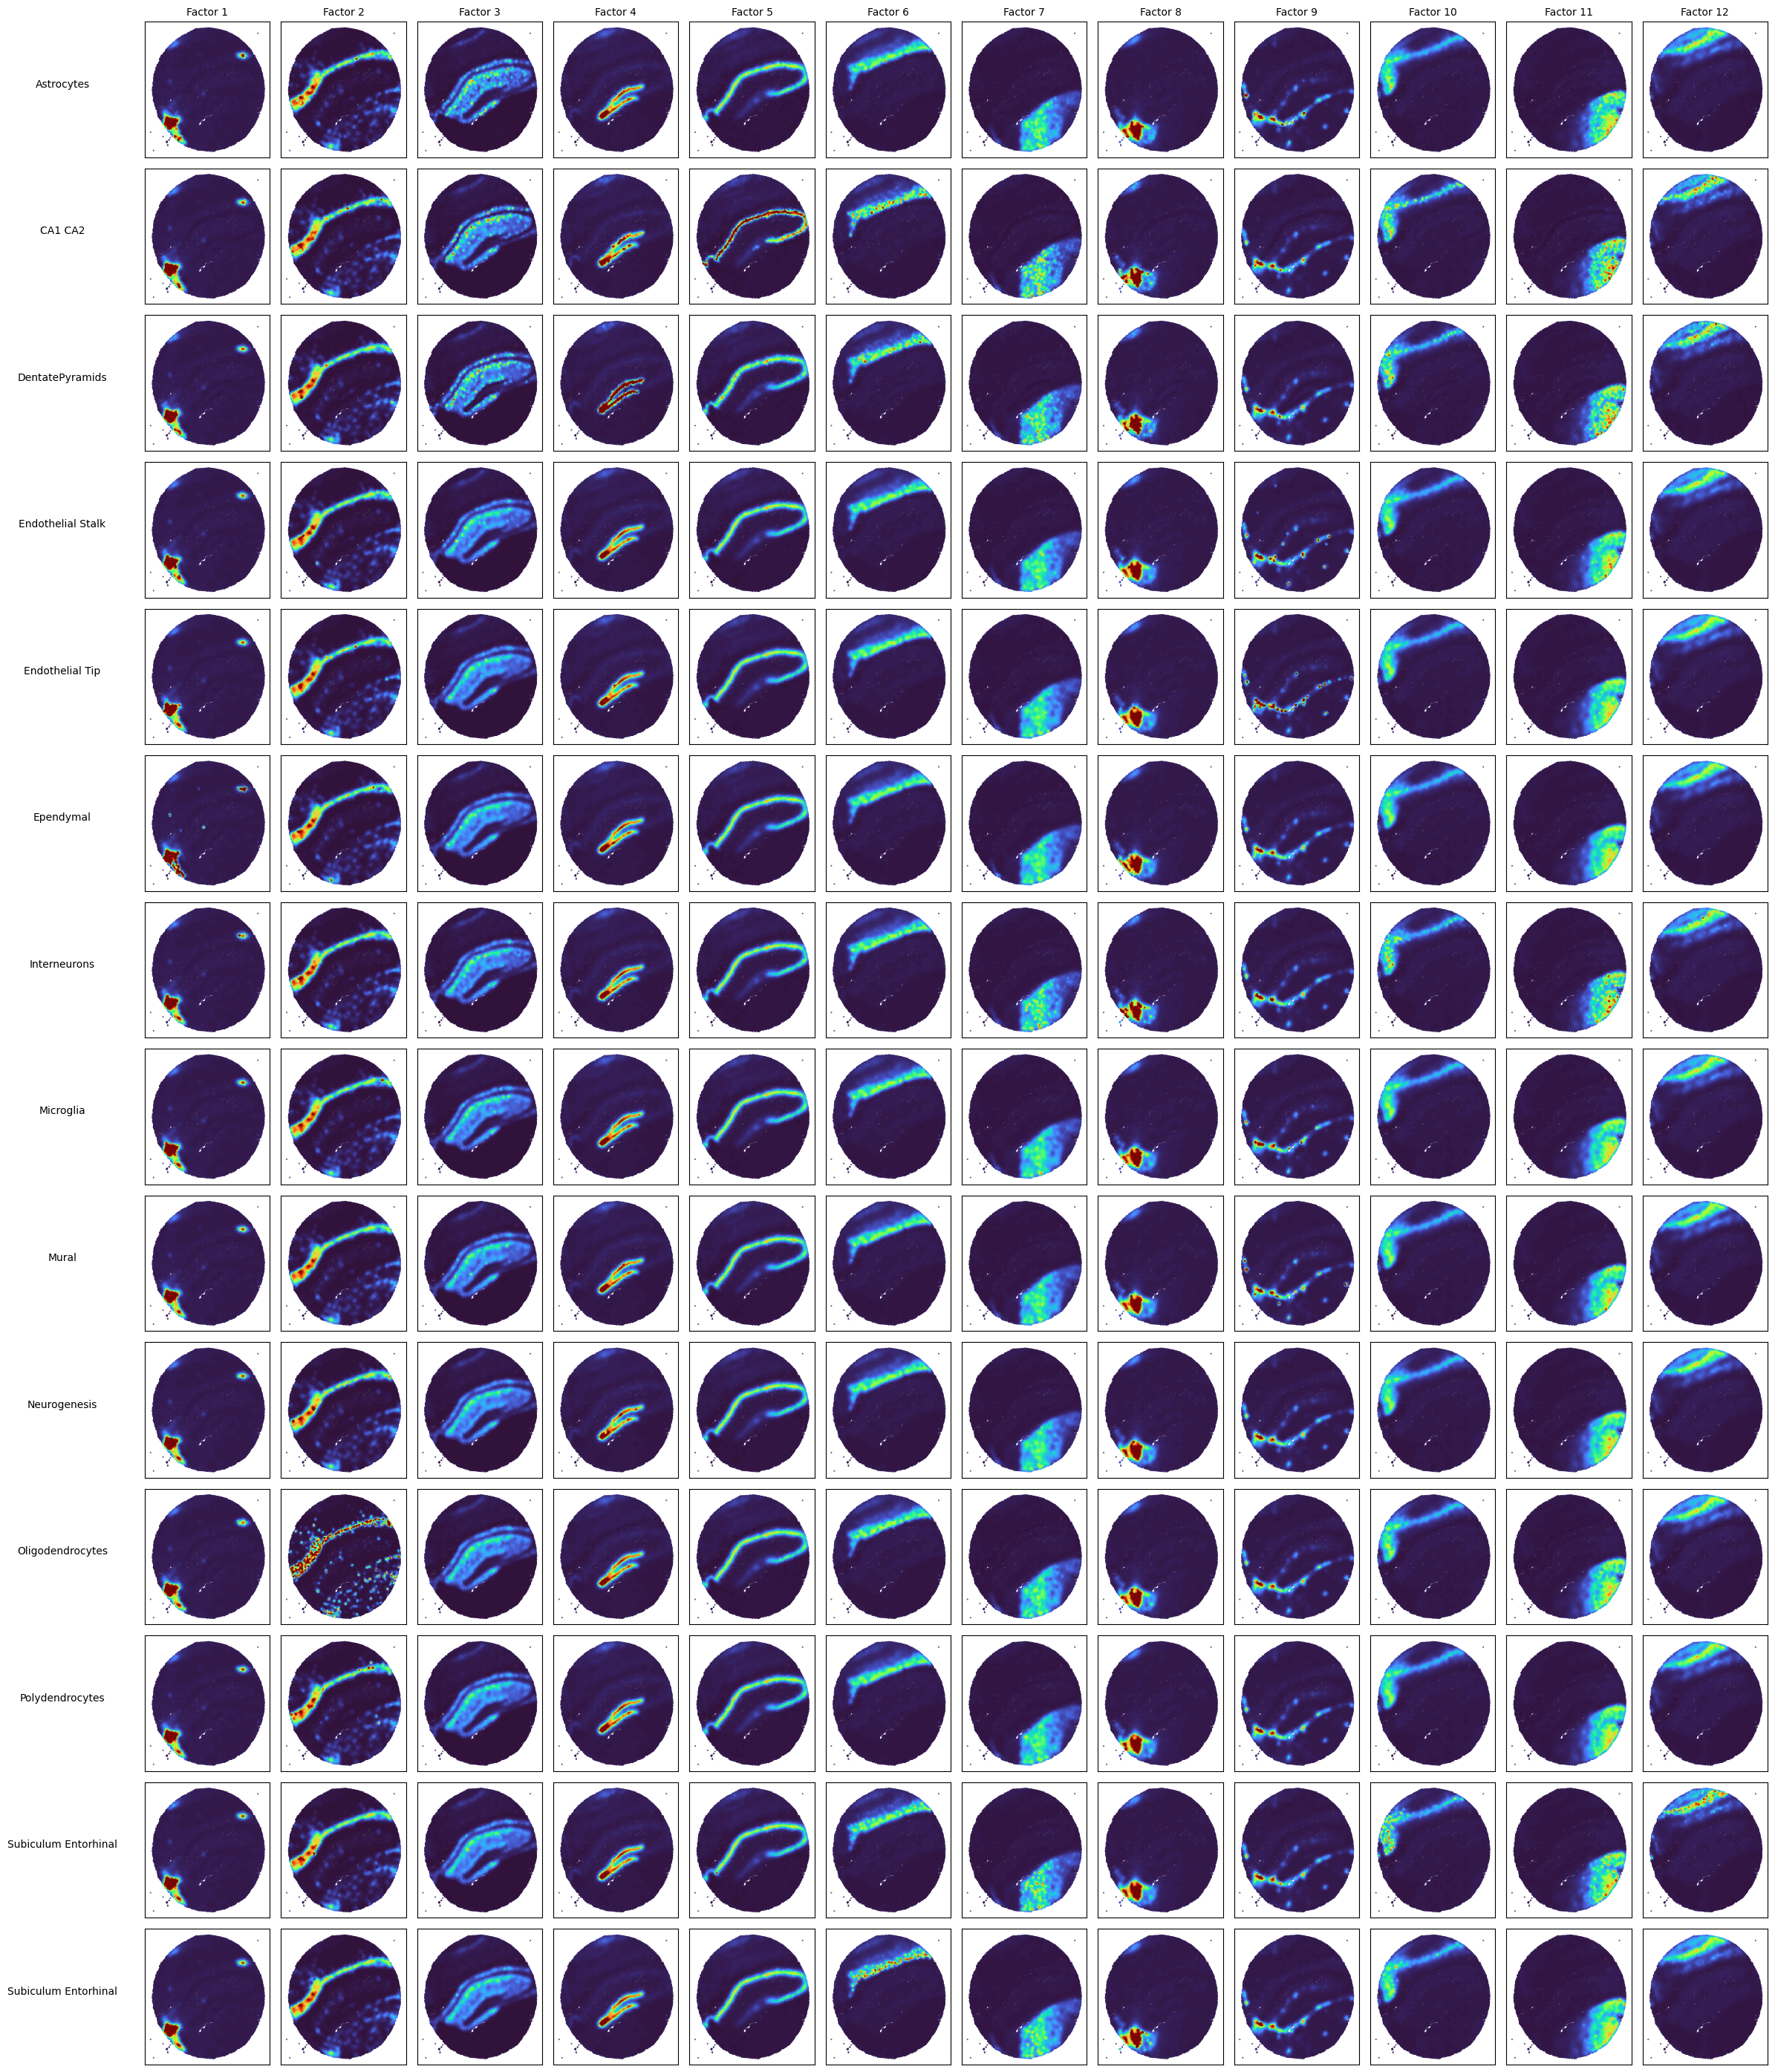
\includegraphics[width=1\textwidth]{Figure4}
\caption{}
% \caption{This is a widefig. This is an example of long caption this is an example of long caption  this is an example of long caption this is an example of long caption}\label{fig1}
\end{figure}



\begin{figure}[H]%
\centering
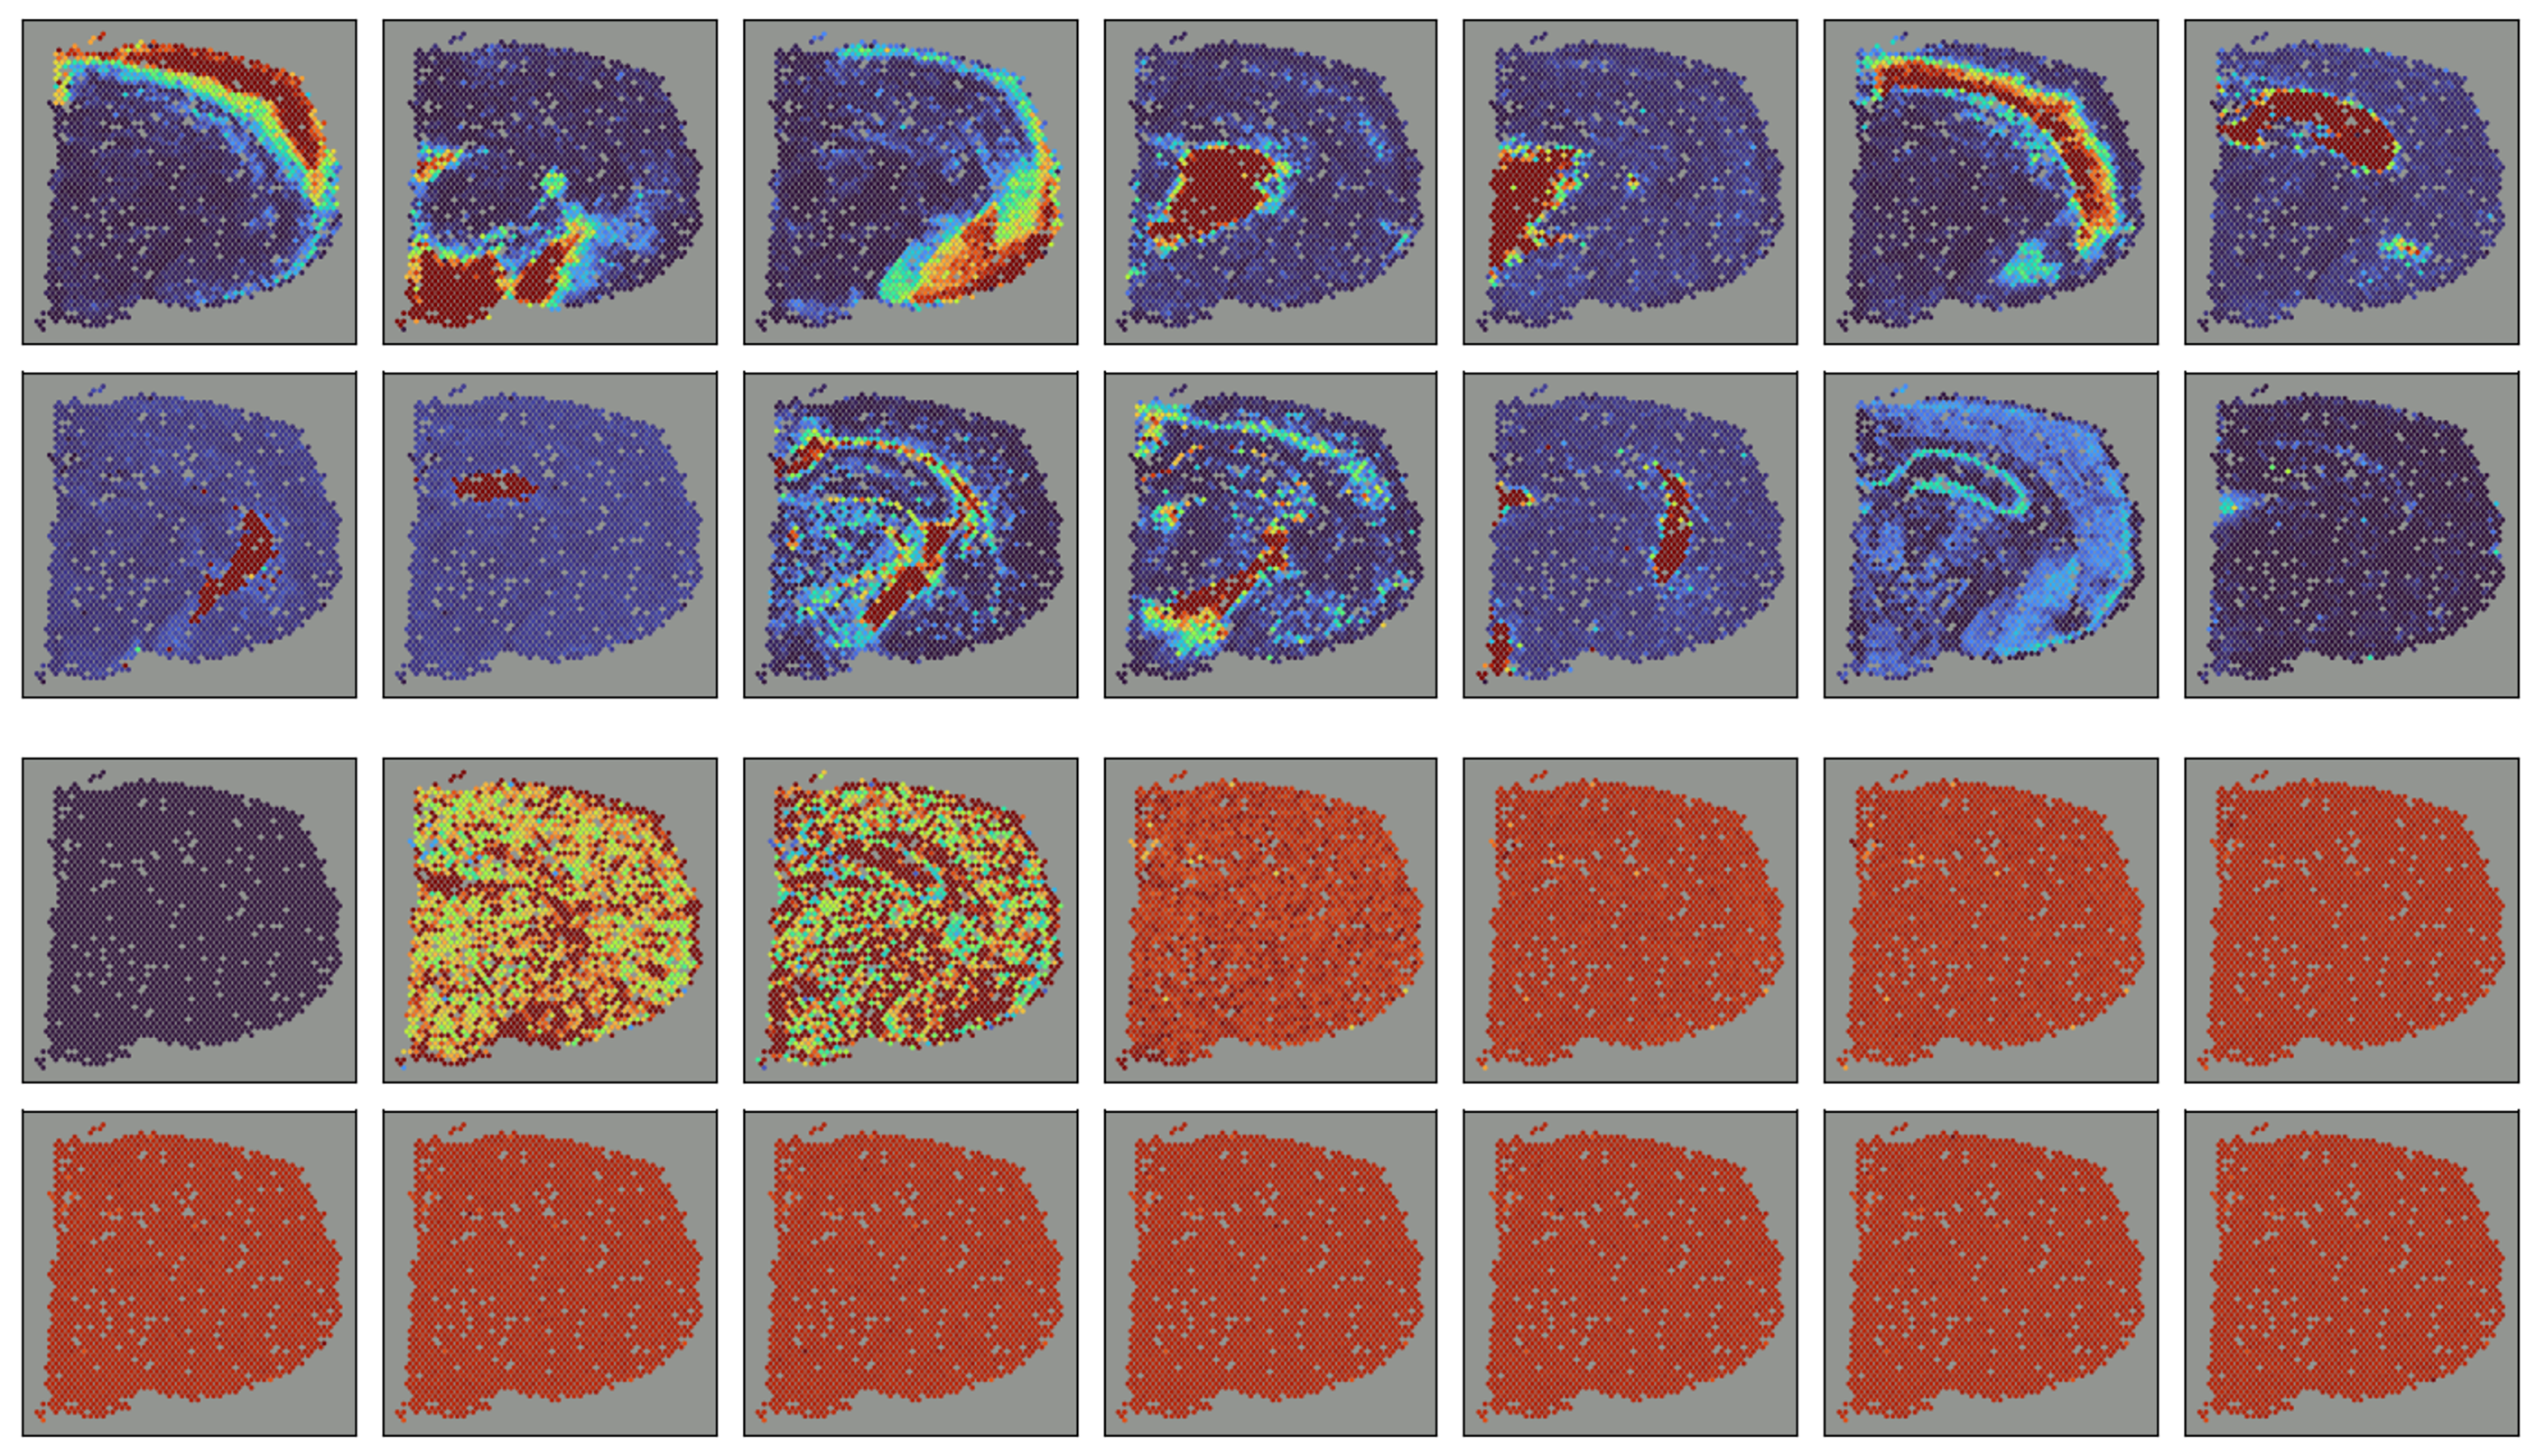
\includegraphics[width=0.7\textwidth]{Figure5}
\caption{}
% \caption{This is a widefig. This is an example of long caption this is an example of long caption  this is an example of long caption this is an example of long caption}\label{fig1}
\end{figure}



\begin{figure}[H]%
\centering
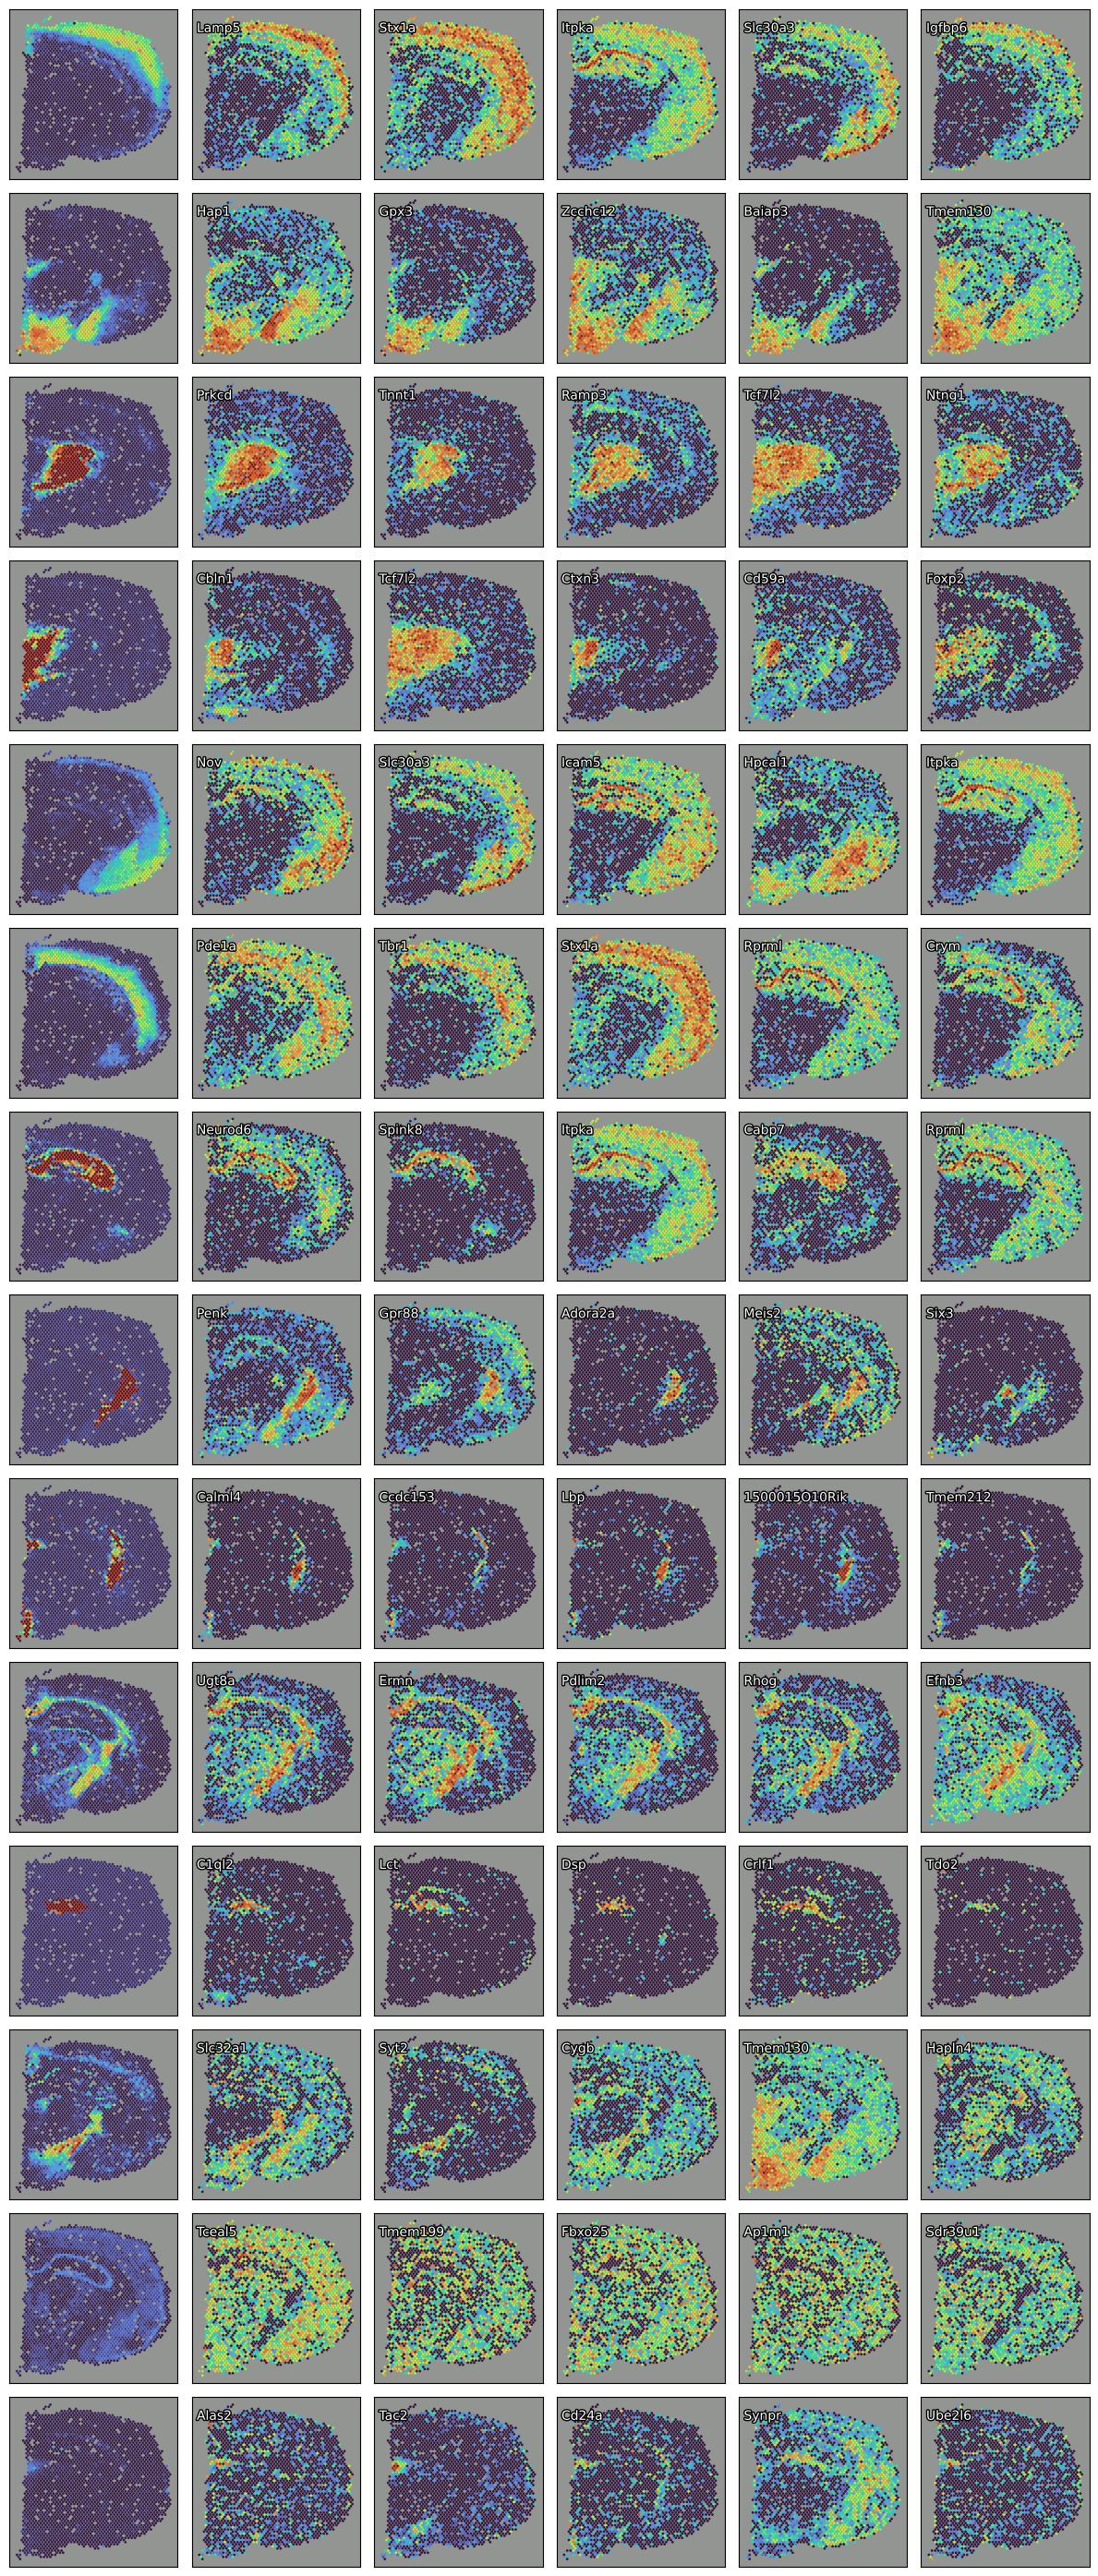
\includegraphics[width=0.8\textwidth]{Figure6}
\caption{}
% \caption{This is a widefig. This is an example of long caption this is an example of long caption  this is an example of long caption this is an example of long caption}\label{fig1}
\end{figure}


\begin{figure}[H]%
\centering
\includegraphics[width=1\textwidth]{Figure7}
\caption{}
% \caption{This is a widefig. This is an example of long caption this is an example of long caption  this is an example of long caption this is an example of long caption}\label{fig1}
\end{figure}


\begin{figure}[H]%
\centering
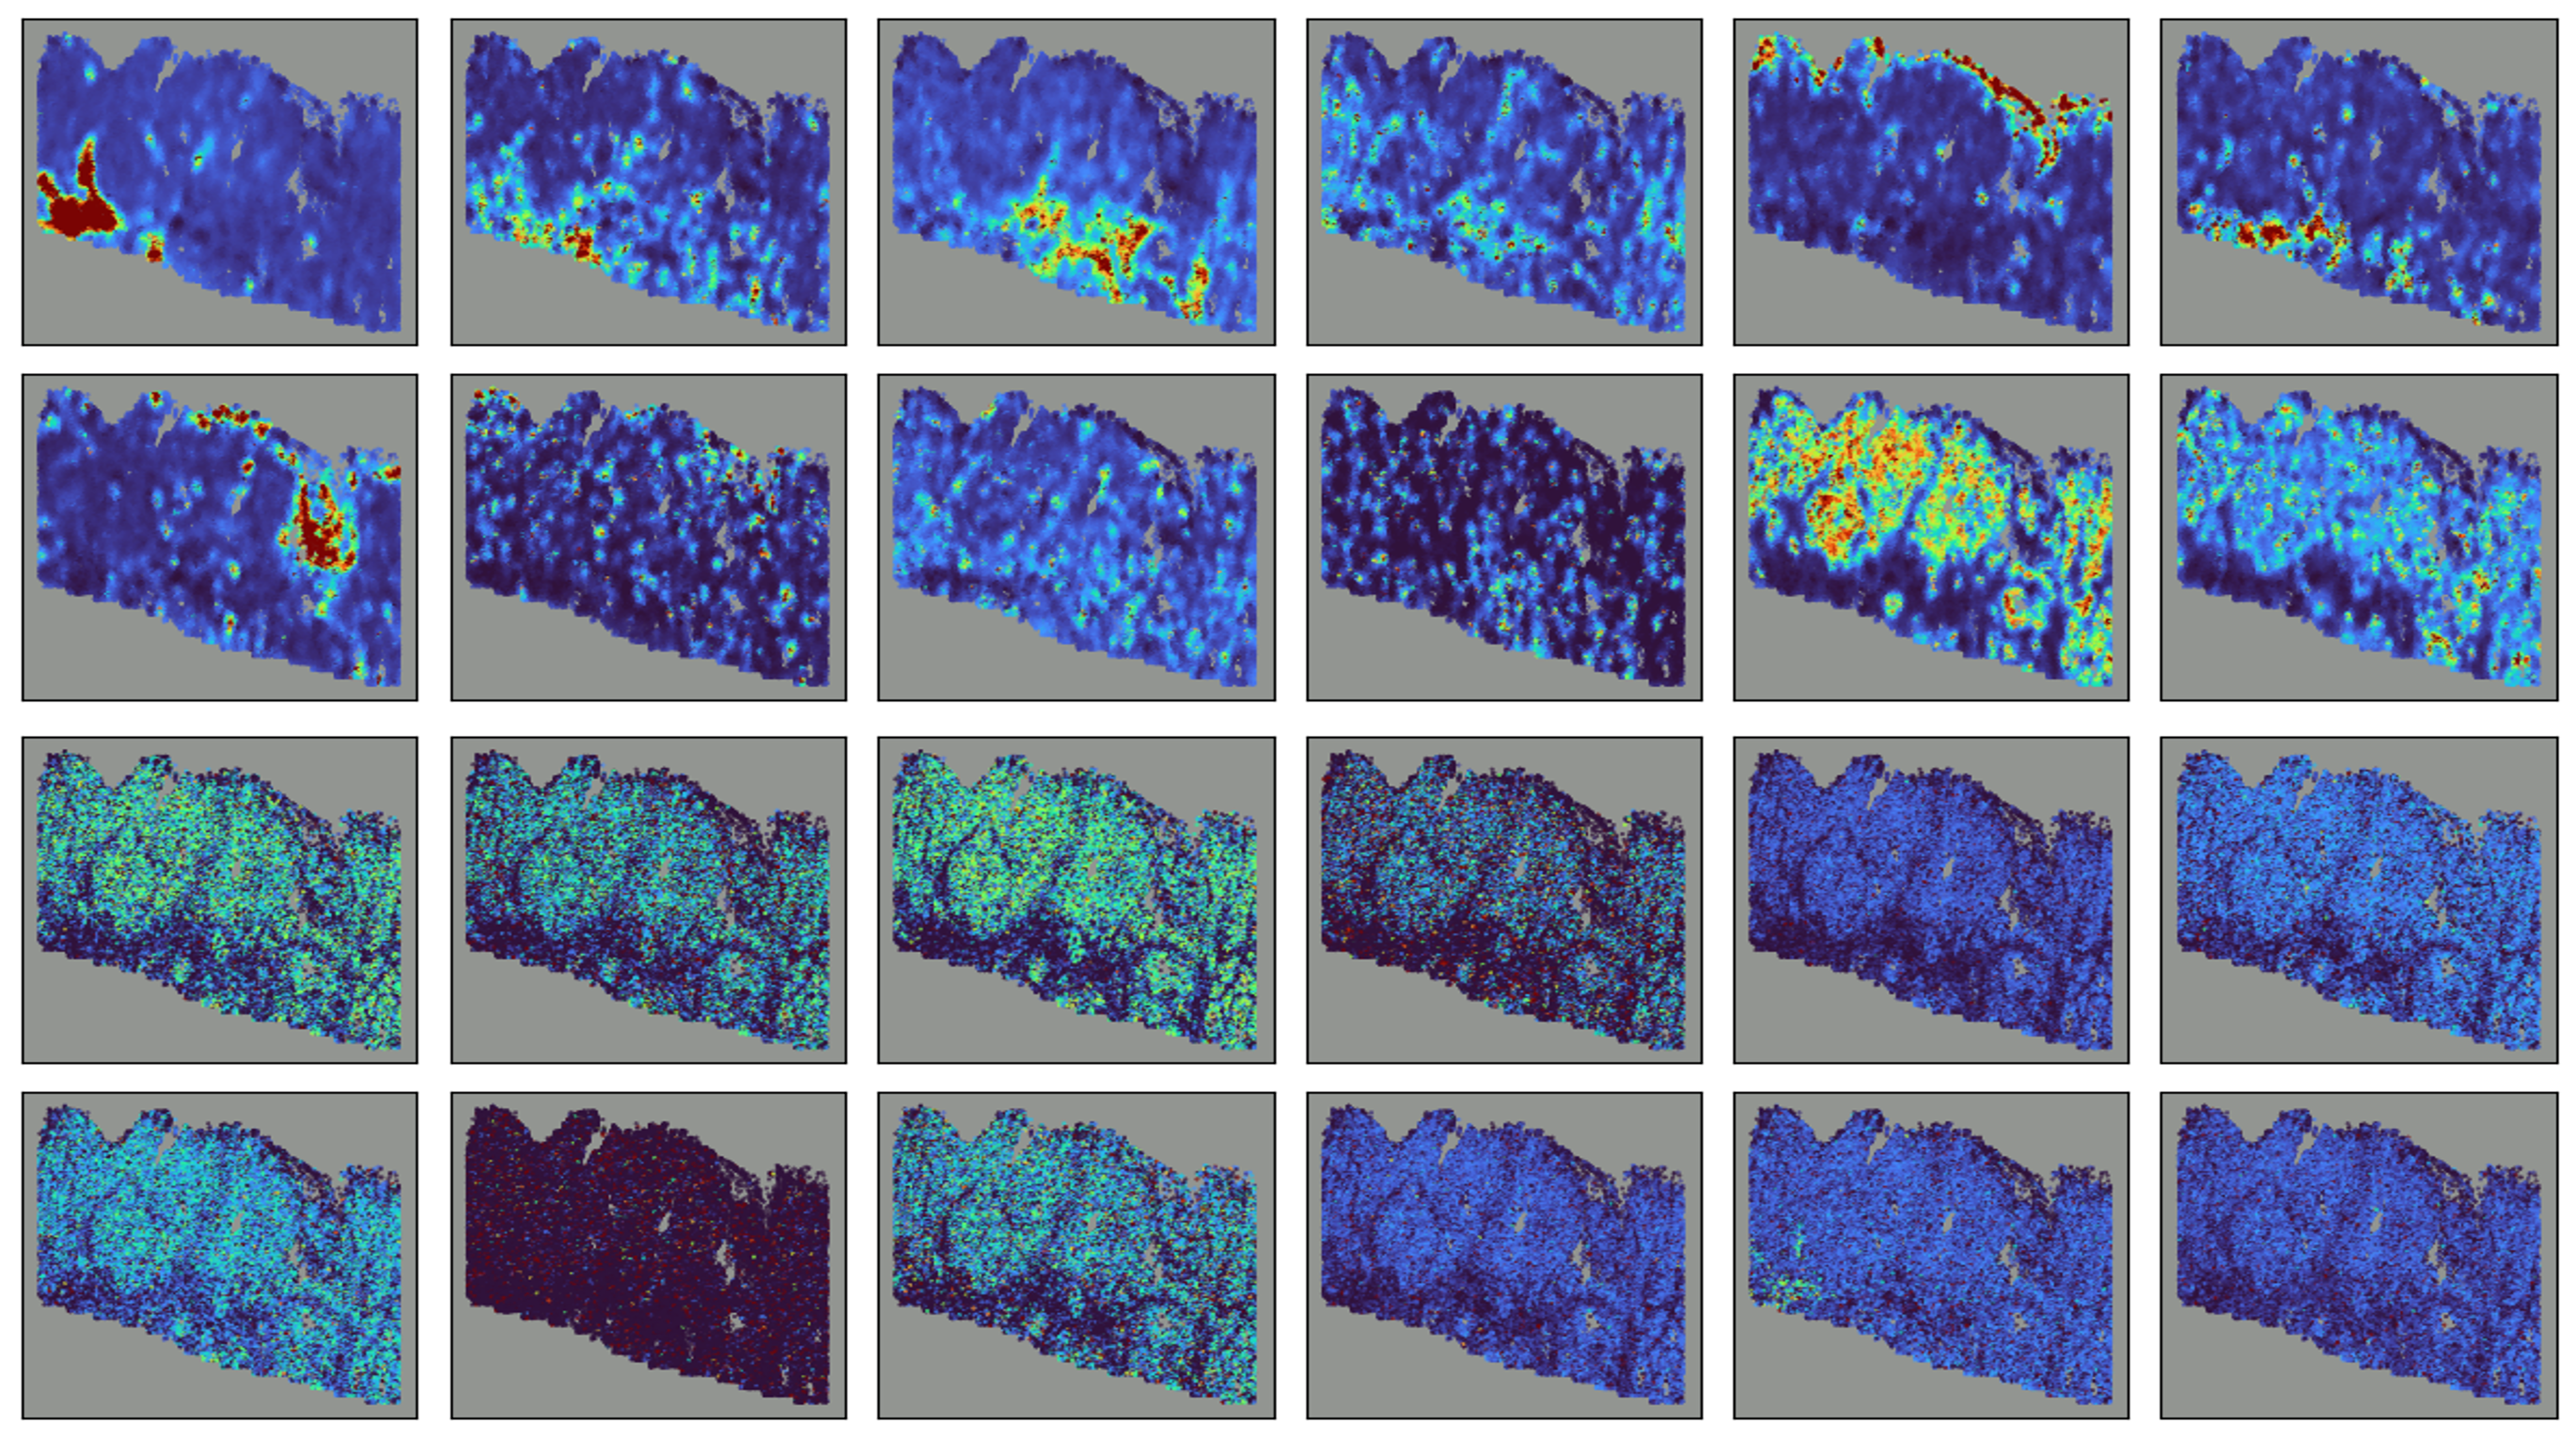
\includegraphics[width=0.7\textwidth]{Figure8}
\caption{}
% \caption{This is a widefig. This is an example of long caption this is an example of long caption  this is an example of long caption this is an example of long caption}\label{fig1}
\end{figure}

\begin{figure}[H]%
\centering
\includegraphics[width=0.9\textwidth]{Figure9}
\caption{}
% \caption{This is a widefig. This is an example of long caption this is an example of long caption  this is an example of long caption this is an example of long caption}\label{fig1}
\end{figure}

\begin{figure}[H]%
\centering
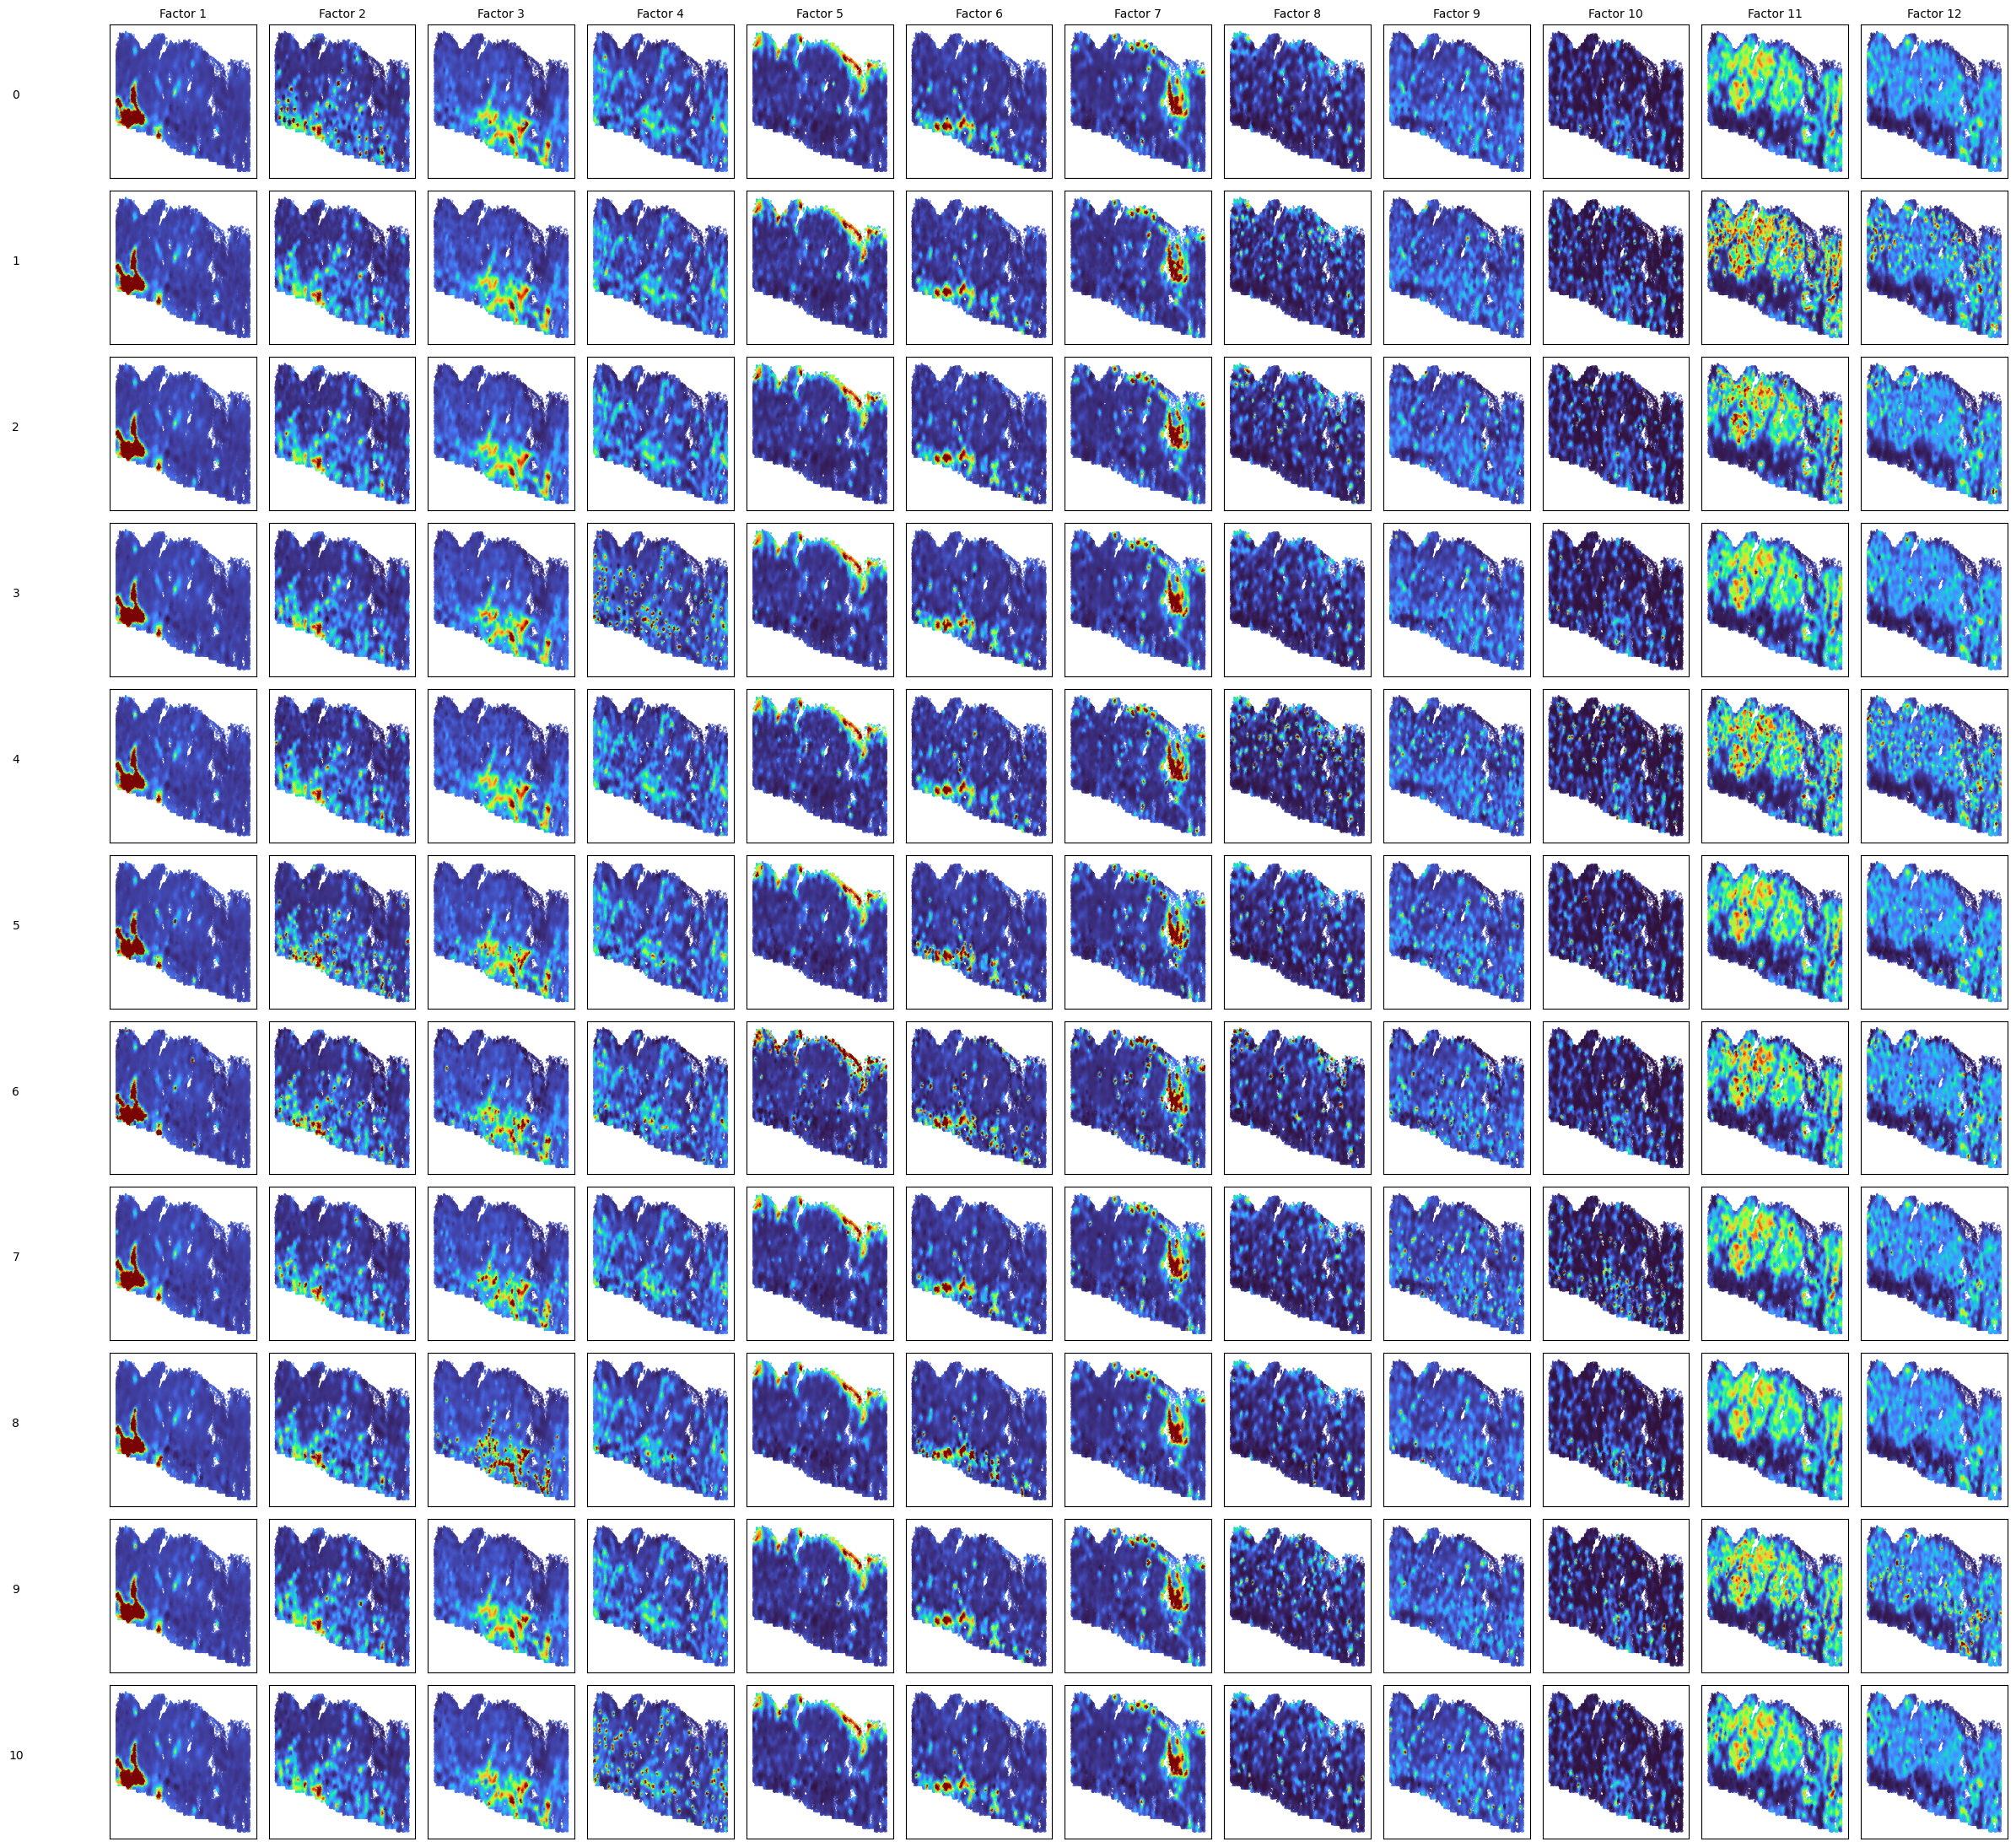
\includegraphics[width=1\textwidth]{Figure10}
\caption{}
% \caption{This is a widefig. This is an example of long caption this is an example of long caption  this is an example of long caption this is an example of long caption}\label{fig1}
\end{figure}



% \section{Conclusion}\label{sec13}

% Conclusions may be used to restate your hypothesis or research question, restate your major findings, explain the relevance and the added value of your work, highlight any limitations of your study, describe future directions for research and recommendations. 

% In some disciplines use of Discussion or 'Conclusion' is interchangeable. It is not mandatory to use both. Please refer to Journal-level guidance for any specific requirements. 



\begin{appendices}

\section{Useful Identities}\label{secA}

In this section we display Gaussian marginalization and the computation of the KL divergence of two Gaussian distributions, both derived in Damianou et al. 2015 \cite{Damianou2015-dy} and Townes et al. 2023 \cite{Townes2023-it} respectively.
\subsection{Gaussian Marginalization}\label{subsecA1}

We start by defining the following distributions:
\[p(f|u) = \mathcal{N}(f| Wu, \Sigma_f)\]
\[p(u) = \mathcal{N}(u| m_u, \Sigma_u)\]

The marginal distribution becomes the following:

\[p(f) = \mathcal{N}(f| Wm_u, \Sigma_f+W\Sigma_{u}W^T)\]
\subsection{KL divergence}\label{subsecA2}

We define the following distributions, where $u \in \mathbb{R}^N$:

\[p(u) = \mathcal{N}(u| \mu, \Sigma)\]
\[q(u) = \mathcal{N}(u| m, S)\]

The closed form of the KL divergence over $q(u)$, becomes:


\[ \text{KL} \left( q(\mathbf{u}) \parallel p(\mathbf{u}) \right) = \frac{1}{2} \left[ \log \frac{|\Sigma|}{|S|} - N + \text{tr} \left\{ \Sigma^{-1} S \right\} + (m - \mu)' \Sigma^{-1} (m - \mu) \right] \]
        

\end{appendices}

%%===========================================================================================%%
%% If you are submitting to one of the Nature Portfolio journals, using the eJP submission   %%
%% system, please include the references within the manuscript file itself. You may do this  %%
%% by copying the reference list from your .bbl file, paste it into the main manuscript .tex %%
%% file, and delete the associated \verb+\bibliography+ commands.                            %%
%%===========================================================================================%%

% \bibliography{sn-bibliography}% common bib file
\bibliography{paperpile}
%% if required, the content of .bbl file can be included here once bbl is generated
%%\input sn-article.bbl


\end{document}
